\documentclass[12pt]{article}
\usepackage[utf8]{inputenc}
\usepackage{pgf,tikz,pgfplots}
\pgfplotsset{compat=1.15}
\usepackage{mathrsfs}
\usetikzlibrary{arrows}
\usepackage{fontspec}
\setmainfont[Renderer=ICU,Mapping=tex-text]{Cousine}
\usepackage{amssymb}
\usepackage[paperwidth=80.96cm,paperheight=44.9cm,left=0.1cm,right=0.1cm,top=0.1cm,bottom=0.1cm]{geometry}
\begin{document}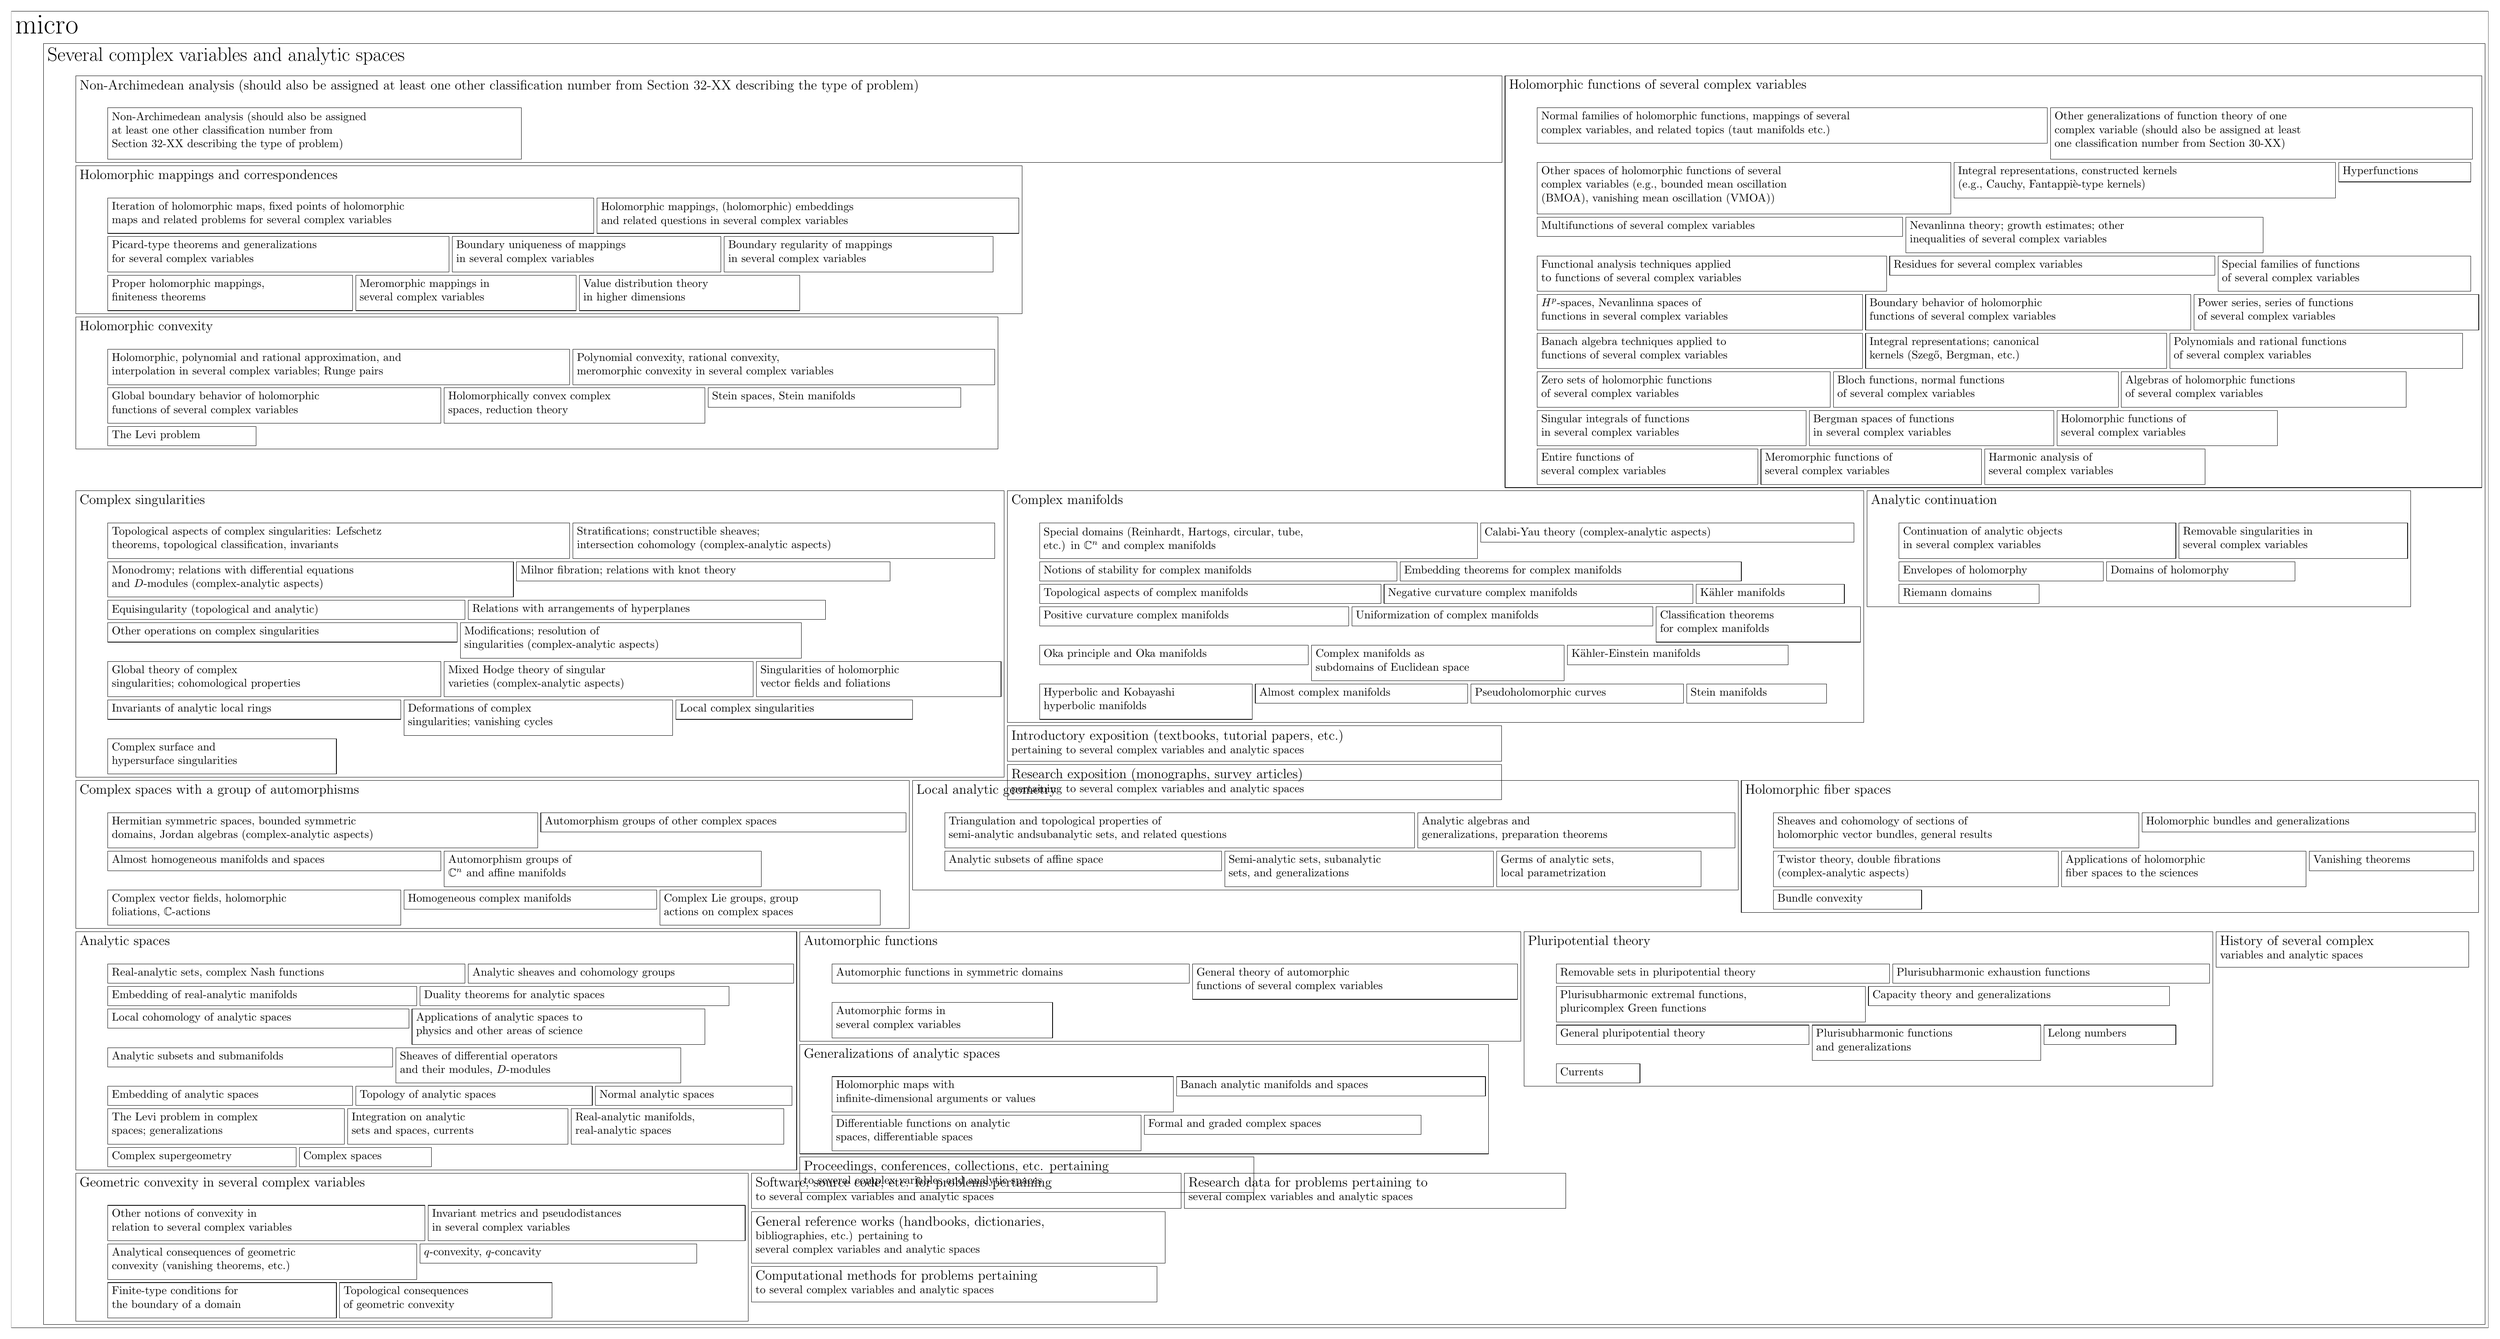
\begin{tikzpicture}[line cap=round,line join=round,>=triangle 45,x=1cm,y=1cm]
\clip(0, 0)rectangle(76.96, -40.9);

\draw(0, 0) node[anchor=north west,align=left] {\Huge micro};
\draw (0, 0) rectangle (76.96,-40.9);
\draw(1, -1) node[anchor=north west,align=left] {\LARGE Several complex variables and analytic spaces};
\draw (1, -1) rectangle (76.86,-40.8);
\draw(2, -2) node[anchor=north west,align=left] {\large Non-Archimedean analysis (should also be assigned at least one other classification number from Section 32-XX describing the type of problem)};
\draw (2, -2) rectangle (46.31,-4.7);
\draw(3, -3) node[anchor=north west,align=left] {Non-Archimedean analysis (should also be assigned\\ at least one other classification number from\\ Section 32-XX describing the type of problem)};
\draw (3, -3) rectangle (15.85,-4.6);
\draw(46.410000000000004, -2) node[anchor=north west,align=left] {\large Holomorphic functions of several complex variables};
\draw (46.410000000000004, -2) rectangle (76.76,-14.799999999999997);
\draw(47.410000000000004, -3) node[anchor=north west,align=left] {Normal families of holomorphic functions, mappings of several\\ complex variables, and related topics (taut manifolds etc.)};
\draw (47.410000000000004, -3) rectangle (63.260000000000005,-4.1);
\draw(63.36000000000001, -3) node[anchor=north west,align=left] {Other generalizations of function theory of one\\ complex variable (should also be assigned at least\\ one classification number from Section 30-XX)};
\draw (63.36000000000001, -3) rectangle (76.46000000000001,-4.6);
\draw(47.410000000000004, -4.7) node[anchor=north west,align=left] {Other spaces of holomorphic functions of several\\ complex variables (e.g., bounded mean oscillation\\ (BMOA), vanishing mean oscillation (VMOA))};
\draw (47.410000000000004, -4.7) rectangle (60.260000000000005,-6.300000000000001);
\draw(60.36, -4.7) node[anchor=north west,align=left] {Integral representations, constructed kernels\\ (e.g., Cauchy, Fantappiè-type kernels)};
\draw (60.36, -4.7) rectangle (72.21,-5.800000000000001);
\draw(72.31, -4.7) node[anchor=north west,align=left] {Hyperfunctions};
\draw (72.31, -4.7) rectangle (76.41,-5.3);
\draw(47.410000000000004, -6.4) node[anchor=north west,align=left] {Multifunctions of several complex variables};
\draw (47.410000000000004, -6.4) rectangle (58.760000000000005,-7.0);
\draw(58.86, -6.4) node[anchor=north west,align=left] {Nevanlinna theory; growth estimates; other\\ inequalities of several complex variables};
\draw (58.86, -6.4) rectangle (69.96,-7.5);
\draw(47.410000000000004, -7.6000000000000005) node[anchor=north west,align=left] {Functional analysis techniques applied \\ to functions of several complex variables};
\draw (47.410000000000004, -7.6000000000000005) rectangle (58.260000000000005,-8.700000000000001);
\draw(58.36, -7.6000000000000005) node[anchor=north west,align=left] {Residues for several complex variables};
\draw (58.36, -7.6000000000000005) rectangle (68.46,-8.200000000000001);
\draw(68.56, -7.6000000000000005) node[anchor=north west,align=left] {Special families of functions\\ of several complex variables};
\draw (68.56, -7.6000000000000005) rectangle (76.41,-8.700000000000001);
\draw(47.410000000000004, -8.8) node[anchor=north west,align=left] {\(H^p\)-spaces, Nevanlinna spaces of\\ functions in several complex variables};
\draw (47.410000000000004, -8.8) rectangle (57.510000000000005,-9.9);
\draw(57.61, -8.8) node[anchor=north west,align=left] {Boundary behavior of holomorphic \\ functions of several complex variables};
\draw (57.61, -8.8) rectangle (67.71,-9.9);
\draw(67.81, -8.8) node[anchor=north west,align=left] {Power series, series of functions\\ of several complex variables};
\draw (67.81, -8.8) rectangle (76.66,-9.9);
\draw(47.410000000000004, -10.0) node[anchor=north west,align=left] {Banach algebra techniques applied to\\ functions of several complex variables};
\draw (47.410000000000004, -10.0) rectangle (57.510000000000005,-11.1);
\draw(57.61, -10.0) node[anchor=north west,align=left] {Integral representations; canonical\\ kernels (Szegő, Bergman, etc.)};
\draw (57.61, -10.0) rectangle (66.96,-11.1);
\draw(67.06, -10.0) node[anchor=north west,align=left] {Polynomials and rational functions\\ of several complex variables};
\draw (67.06, -10.0) rectangle (76.16,-11.1);
\draw(47.410000000000004, -11.2) node[anchor=north west,align=left] {Zero sets of holomorphic functions\\ of several complex variables};
\draw (47.410000000000004, -11.2) rectangle (56.510000000000005,-12.299999999999999);
\draw(56.61, -11.2) node[anchor=north west,align=left] {Bloch functions, normal functions\\ of several complex variables};
\draw (56.61, -11.2) rectangle (65.46,-12.299999999999999);
\draw(65.56, -11.2) node[anchor=north west,align=left] {Algebras of holomorphic functions\\ of several complex variables};
\draw (65.56, -11.2) rectangle (74.41,-12.299999999999999);
\draw(47.410000000000004, -12.399999999999999) node[anchor=north west,align=left] {Singular integrals of functions\\ in several complex variables};
\draw (47.410000000000004, -12.399999999999999) rectangle (55.760000000000005,-13.499999999999998);
\draw(55.86, -12.399999999999999) node[anchor=north west,align=left] {Bergman spaces of functions\\ in several complex variables};
\draw (55.86, -12.399999999999999) rectangle (63.46,-13.499999999999998);
\draw(63.56, -12.399999999999999) node[anchor=north west,align=left] {Holomorphic functions of\\ several complex variables};
\draw (63.56, -12.399999999999999) rectangle (70.41,-13.499999999999998);
\draw(47.410000000000004, -13.599999999999998) node[anchor=north west,align=left] {Entire functions of \\ several complex variables};
\draw (47.410000000000004, -13.599999999999998) rectangle (54.260000000000005,-14.699999999999998);
\draw(54.36, -13.599999999999998) node[anchor=north west,align=left] {Meromorphic functions of\\ several complex variables};
\draw (54.36, -13.599999999999998) rectangle (61.21,-14.699999999999998);
\draw(61.31, -13.599999999999998) node[anchor=north west,align=left] {Harmonic analysis of \\ several complex variables};
\draw (61.31, -13.599999999999998) rectangle (68.16,-14.699999999999998);
\draw(2, -4.800000000000001) node[anchor=north west,align=left] {\large Holomorphic mappings and correspondences};
\draw (2, -4.800000000000001) rectangle (31.400000000000006,-9.4);
\draw(3, -5.800000000000001) node[anchor=north west,align=left] {Iteration of holomorphic maps, fixed points of holomorphic\\ maps and related problems for several complex variables};
\draw (3, -5.800000000000001) rectangle (18.1,-6.9);
\draw(18.200000000000003, -5.800000000000001) node[anchor=north west,align=left] {Holomorphic mappings, (holomorphic) embeddings \\ and related questions in several complex variables};
\draw (18.200000000000003, -5.800000000000001) rectangle (31.300000000000004,-6.9);
\draw(3, -7.000000000000001) node[anchor=north west,align=left] {Picard-type theorems and generalizations\\ for several complex variables};
\draw (3, -7.000000000000001) rectangle (13.6,-8.100000000000001);
\draw(13.7, -7.000000000000001) node[anchor=north west,align=left] {Boundary uniqueness of mappings\\ in several complex variables};
\draw (13.7, -7.000000000000001) rectangle (22.049999999999997,-8.100000000000001);
\draw(22.15, -7.000000000000001) node[anchor=north west,align=left] {Boundary regularity of mappings\\ in several complex variables};
\draw (22.15, -7.000000000000001) rectangle (30.5,-8.100000000000001);
\draw(3, -8.200000000000001) node[anchor=north west,align=left] {Proper holomorphic mappings,\\ finiteness theorems};
\draw (3, -8.200000000000001) rectangle (10.6,-9.3);
\draw(10.7, -8.200000000000001) node[anchor=north west,align=left] {Meromorphic mappings in\\ several complex variables};
\draw (10.7, -8.200000000000001) rectangle (17.549999999999997,-9.3);
\draw(17.65, -8.200000000000001) node[anchor=north west,align=left] {Value distribution theory\\ in higher dimensions};
\draw (17.65, -8.200000000000001) rectangle (24.5,-9.3);
\draw(2, -9.499999999999998) node[anchor=north west,align=left] {\large Holomorphic convexity};
\draw (2, -9.499999999999998) rectangle (30.65,-13.599999999999998);
\draw(3, -10.499999999999998) node[anchor=north west,align=left] {Holomorphic, polynomial and rational approximation, and\\ interpolation in several complex variables; Runge pairs};
\draw (3, -10.499999999999998) rectangle (17.35,-11.599999999999998);
\draw(17.45, -10.499999999999998) node[anchor=north west,align=left] {Polynomial convexity, rational convexity, \\ meromorphic convexity in several complex variables};
\draw (17.45, -10.499999999999998) rectangle (30.549999999999997,-11.599999999999998);
\draw(3, -11.7) node[anchor=north west,align=left] {Global boundary behavior of holomorphic\\ functions of several complex variables};
\draw (3, -11.7) rectangle (13.35,-12.799999999999999);
\draw(13.45, -11.7) node[anchor=north west,align=left] {Holomorphically convex complex\\ spaces, reduction theory};
\draw (13.45, -11.7) rectangle (21.549999999999997,-12.799999999999999);
\draw(21.65, -11.7) node[anchor=north west,align=left] {Stein spaces, Stein manifolds};
\draw (21.65, -11.7) rectangle (29.5,-12.299999999999999);
\draw(3, -12.899999999999999) node[anchor=north west,align=left] {The Levi problem};
\draw (3, -12.899999999999999) rectangle (7.6,-13.499999999999998);
\draw(2, -14.899999999999997) node[anchor=north west,align=left] {\large Complex singularities};
\draw (2, -14.899999999999997) rectangle (30.85,-23.799999999999997);
\draw(3, -15.899999999999997) node[anchor=north west,align=left] {Topological aspects of complex singularities: Lefschetz\\ theorems, topological classification, invariants};
\draw (3, -15.899999999999997) rectangle (17.35,-16.999999999999996);
\draw(17.45, -15.899999999999997) node[anchor=north west,align=left] {Stratifications; constructible sheaves; \\ intersection cohomology (complex-analytic aspects)};
\draw (17.45, -15.899999999999997) rectangle (30.549999999999997,-16.999999999999996);
\draw(3, -17.099999999999998) node[anchor=north west,align=left] {Monodromy; relations with differential equations\\ and \(D\)-modules (complex-analytic aspects)};
\draw (3, -17.099999999999998) rectangle (15.6,-18.2);
\draw(15.7, -17.099999999999998) node[anchor=north west,align=left] {Milnor fibration; relations with knot theory};
\draw (15.7, -17.099999999999998) rectangle (27.299999999999997,-17.7);
\draw(3, -18.299999999999997) node[anchor=north west,align=left] {Equisingularity (topological and analytic)};
\draw (3, -18.299999999999997) rectangle (14.1,-18.9);
\draw(14.2, -18.299999999999997) node[anchor=north west,align=left] {Relations with arrangements of hyperplanes};
\draw (14.2, -18.299999999999997) rectangle (25.299999999999997,-18.9);
\draw(3, -18.999999999999996) node[anchor=north west,align=left] {Other operations on complex singularities};
\draw (3, -18.999999999999996) rectangle (13.85,-19.599999999999998);
\draw(13.95, -18.999999999999996) node[anchor=north west,align=left] {Modifications; resolution of \\ singularities (complex-analytic aspects)};
\draw (13.95, -18.999999999999996) rectangle (24.549999999999997,-20.099999999999998);
\draw(3, -20.199999999999996) node[anchor=north west,align=left] {Global theory of complex \\ singularities; cohomological properties};
\draw (3, -20.199999999999996) rectangle (13.35,-21.299999999999997);
\draw(13.45, -20.199999999999996) node[anchor=north west,align=left] {Mixed Hodge theory of singular \\ varieties (complex-analytic aspects)};
\draw (13.45, -20.199999999999996) rectangle (23.049999999999997,-21.299999999999997);
\draw(23.15, -20.199999999999996) node[anchor=north west,align=left] {Singularities of holomorphic\\ vector fields and foliations};
\draw (23.15, -20.199999999999996) rectangle (30.75,-21.299999999999997);
\draw(3, -21.4) node[anchor=north west,align=left] {Invariants of analytic local rings};
\draw (3, -21.4) rectangle (12.1,-22.0);
\draw(12.2, -21.4) node[anchor=north west,align=left] {Deformations of complex \\ singularities; vanishing cycles};
\draw (12.2, -21.4) rectangle (20.549999999999997,-22.5);
\draw(20.65, -21.4) node[anchor=north west,align=left] {Local complex singularities};
\draw (20.65, -21.4) rectangle (28.0,-22.0);
\draw(3, -22.599999999999998) node[anchor=north west,align=left] {Complex surface and \\ hypersurface singularities};
\draw (3, -22.599999999999998) rectangle (10.1,-23.7);
\draw(30.950000000000003, -14.899999999999997) node[anchor=north west,align=left] {\large Complex manifolds};
\draw (30.950000000000003, -14.899999999999997) rectangle (57.550000000000004,-22.099999999999998);
\draw(31.950000000000003, -15.899999999999997) node[anchor=north west,align=left] {Special domains (Reinhardt, Hartogs, circular, tube,\\ etc.) in \(\mathbb{C}^n\) and complex manifolds};
\draw (31.950000000000003, -15.899999999999997) rectangle (45.550000000000004,-16.999999999999996);
\draw(45.650000000000006, -15.899999999999997) node[anchor=north west,align=left] {Calabi-Yau theory (complex-analytic aspects)};
\draw (45.650000000000006, -15.899999999999997) rectangle (57.25000000000001,-16.499999999999996);
\draw(31.950000000000003, -17.099999999999998) node[anchor=north west,align=left] {Notions of stability for complex manifolds};
\draw (31.950000000000003, -17.099999999999998) rectangle (43.050000000000004,-17.7);
\draw(43.150000000000006, -17.099999999999998) node[anchor=north west,align=left] {Embedding theorems for complex manifolds};
\draw (43.150000000000006, -17.099999999999998) rectangle (53.75000000000001,-17.7);
\draw(31.950000000000003, -17.799999999999997) node[anchor=north west,align=left] {Topological aspects of complex manifolds};
\draw (31.950000000000003, -17.799999999999997) rectangle (42.550000000000004,-18.4);
\draw(42.650000000000006, -17.799999999999997) node[anchor=north west,align=left] {Negative curvature complex manifolds};
\draw (42.650000000000006, -17.799999999999997) rectangle (52.25000000000001,-18.4);
\draw(52.35, -17.799999999999997) node[anchor=north west,align=left] {Kähler manifolds};
\draw (52.35, -17.799999999999997) rectangle (56.95,-18.4);
\draw(31.950000000000003, -18.499999999999996) node[anchor=north west,align=left] {Positive curvature complex manifolds};
\draw (31.950000000000003, -18.499999999999996) rectangle (41.550000000000004,-19.099999999999998);
\draw(41.650000000000006, -18.499999999999996) node[anchor=north west,align=left] {Uniformization of complex manifolds};
\draw (41.650000000000006, -18.499999999999996) rectangle (51.00000000000001,-19.099999999999998);
\draw(51.1, -18.499999999999996) node[anchor=north west,align=left] {Classification theorems\\ for complex manifolds};
\draw (51.1, -18.499999999999996) rectangle (57.45,-19.599999999999998);
\draw(31.950000000000003, -19.699999999999996) node[anchor=north west,align=left] {Oka principle and Oka manifolds};
\draw (31.950000000000003, -19.699999999999996) rectangle (40.300000000000004,-20.299999999999997);
\draw(40.400000000000006, -19.699999999999996) node[anchor=north west,align=left] {Complex manifolds as \\ subdomains of Euclidean space};
\draw (40.400000000000006, -19.699999999999996) rectangle (48.25000000000001,-20.799999999999997);
\draw(48.35, -19.699999999999996) node[anchor=north west,align=left] {Kähler-Einstein manifolds};
\draw (48.35, -19.699999999999996) rectangle (55.2,-20.299999999999997);
\draw(31.950000000000003, -20.9) node[anchor=north west,align=left] {Hyperbolic and Kobayashi\\ hyperbolic manifolds};
\draw (31.950000000000003, -20.9) rectangle (38.550000000000004,-22.0);
\draw(38.650000000000006, -20.9) node[anchor=north west,align=left] {Almost complex manifolds};
\draw (38.650000000000006, -20.9) rectangle (45.25000000000001,-21.5);
\draw(45.35, -20.9) node[anchor=north west,align=left] {Pseudoholomorphic curves};
\draw (45.35, -20.9) rectangle (51.95,-21.5);
\draw(52.050000000000004, -20.9) node[anchor=north west,align=left] {Stein manifolds};
\draw (52.050000000000004, -20.9) rectangle (56.400000000000006,-21.5);
\draw(30.950000000000003, -22.2) node[anchor=north west,align=left] {\large Introductory exposition (textbooks, tutorial papers, etc.)\\ pertaining to several complex variables and analytic spaces};
\draw (30.950000000000003, -22.2) rectangle (46.300000000000004,-23.3);
\draw(57.650000000000006, -14.899999999999997) node[anchor=north west,align=left] {\large Analytic continuation};
\draw (57.650000000000006, -14.899999999999997) rectangle (74.55000000000001,-18.499999999999996);
\draw(58.650000000000006, -15.899999999999997) node[anchor=north west,align=left] {Continuation of analytic objects\\ in several complex variables};
\draw (58.650000000000006, -15.899999999999997) rectangle (67.25,-16.999999999999996);
\draw(67.35000000000001, -15.899999999999997) node[anchor=north west,align=left] {Removable singularities in\\ several complex variables};
\draw (67.35000000000001, -15.899999999999997) rectangle (74.45,-16.999999999999996);
\draw(58.650000000000006, -17.099999999999998) node[anchor=north west,align=left] {Envelopes of holomorphy};
\draw (58.650000000000006, -17.099999999999998) rectangle (65.0,-17.7);
\draw(65.10000000000001, -17.099999999999998) node[anchor=north west,align=left] {Domains of holomorphy};
\draw (65.10000000000001, -17.099999999999998) rectangle (70.95,-17.7);
\draw(58.650000000000006, -17.799999999999997) node[anchor=north west,align=left] {Riemann domains};
\draw (58.650000000000006, -17.799999999999997) rectangle (63.00000000000001,-18.4);
\draw(30.950000000000003, -23.400000000000002) node[anchor=north west,align=left] {\large Research exposition (monographs, survey articles) \\ pertaining to several complex variables and analytic spaces};
\draw (30.950000000000003, -23.400000000000002) rectangle (46.300000000000004,-24.500000000000004);
\draw(2, -23.9) node[anchor=north west,align=left] {\large Complex spaces with a group of automorphisms};
\draw (2, -23.9) rectangle (27.9,-28.5);
\draw(3, -24.9) node[anchor=north west,align=left] {Hermitian symmetric spaces, bounded symmetric \\ domains, Jordan algebras (complex-analytic aspects)};
\draw (3, -24.9) rectangle (16.35,-26.0);
\draw(16.45, -24.9) node[anchor=north west,align=left] {Automorphism groups of other complex spaces};
\draw (16.45, -24.9) rectangle (27.799999999999997,-25.5);
\draw(3, -26.099999999999998) node[anchor=north west,align=left] {Almost homogeneous manifolds and spaces};
\draw (3, -26.099999999999998) rectangle (13.35,-26.7);
\draw(13.45, -26.099999999999998) node[anchor=north west,align=left] {Automorphism groups of \\ \(\mathbb{C}^n\) and affine manifolds};
\draw (13.45, -26.099999999999998) rectangle (23.299999999999997,-27.2);
\draw(3, -27.299999999999997) node[anchor=north west,align=left] {Complex vector fields, holomorphic\\ foliations, \(\mathbb{C}\)-actions};
\draw (3, -27.299999999999997) rectangle (12.1,-28.4);
\draw(12.2, -27.299999999999997) node[anchor=north west,align=left] {Homogeneous complex manifolds};
\draw (12.2, -27.299999999999997) rectangle (20.049999999999997,-27.9);
\draw(20.15, -27.299999999999997) node[anchor=north west,align=left] {Complex Lie groups, group\\ actions on complex spaces};
\draw (20.15, -27.299999999999997) rectangle (27.0,-28.4);
\draw(28.0, -23.9) node[anchor=north west,align=left] {\large Local analytic geometry};
\draw (28.0, -23.9) rectangle (53.65,-27.299999999999997);
\draw(29.0, -24.9) node[anchor=north west,align=left] {Triangulation and topological properties of \\ semi-analytic andsubanalytic sets, and related questions};
\draw (29.0, -24.9) rectangle (43.6,-26.0);
\draw(43.7, -24.9) node[anchor=north west,align=left] {Analytic algebras and \\ generalizations, preparation theorems};
\draw (43.7, -24.9) rectangle (53.550000000000004,-26.0);
\draw(29.0, -26.099999999999998) node[anchor=north west,align=left] {Analytic subsets of affine space};
\draw (29.0, -26.099999999999998) rectangle (37.6,-26.7);
\draw(37.7, -26.099999999999998) node[anchor=north west,align=left] {Semi-analytic sets, subanalytic\\ sets, and generalizations};
\draw (37.7, -26.099999999999998) rectangle (46.050000000000004,-27.2);
\draw(46.15, -26.099999999999998) node[anchor=north west,align=left] {Germs of analytic sets,\\ local parametrization};
\draw (46.15, -26.099999999999998) rectangle (52.5,-27.2);
\draw(53.75, -23.9) node[anchor=north west,align=left] {\large Holomorphic fiber spaces};
\draw (53.75, -23.9) rectangle (76.65,-28.0);
\draw(54.75, -24.9) node[anchor=north west,align=left] {Sheaves and cohomology of sections of \\ holomorphic vector bundles, general results};
\draw (54.75, -24.9) rectangle (66.1,-26.0);
\draw(66.2, -24.9) node[anchor=north west,align=left] {Holomorphic bundles and generalizations};
\draw (66.2, -24.9) rectangle (76.55,-25.5);
\draw(54.75, -26.099999999999998) node[anchor=north west,align=left] {Twistor theory, double fibrations\\ (complex-analytic aspects)};
\draw (54.75, -26.099999999999998) rectangle (63.6,-27.2);
\draw(63.7, -26.099999999999998) node[anchor=north west,align=left] {Applications of holomorphic\\ fiber spaces to the sciences};
\draw (63.7, -26.099999999999998) rectangle (71.3,-27.2);
\draw(71.4, -26.099999999999998) node[anchor=north west,align=left] {Vanishing theorems};
\draw (71.4, -26.099999999999998) rectangle (76.5,-26.7);
\draw(54.75, -27.299999999999997) node[anchor=north west,align=left] {Bundle convexity};
\draw (54.75, -27.299999999999997) rectangle (59.35,-27.9);
\draw(2, -28.599999999999998) node[anchor=north west,align=left] {\large Analytic spaces};
\draw (2, -28.599999999999998) rectangle (24.4,-36.0);
\draw(3, -29.599999999999998) node[anchor=north west,align=left] {Real-analytic sets, complex Nash functions};
\draw (3, -29.599999999999998) rectangle (14.1,-30.2);
\draw(14.2, -29.599999999999998) node[anchor=north west,align=left] {Analytic sheaves and cohomology groups};
\draw (14.2, -29.599999999999998) rectangle (24.299999999999997,-30.2);
\draw(3, -30.299999999999997) node[anchor=north west,align=left] {Embedding of real-analytic manifolds};
\draw (3, -30.299999999999997) rectangle (12.6,-30.9);
\draw(12.7, -30.299999999999997) node[anchor=north west,align=left] {Duality theorems for analytic spaces};
\draw (12.7, -30.299999999999997) rectangle (22.299999999999997,-30.9);
\draw(3, -30.999999999999996) node[anchor=north west,align=left] {Local cohomology of analytic spaces};
\draw (3, -30.999999999999996) rectangle (12.35,-31.599999999999998);
\draw(12.45, -30.999999999999996) node[anchor=north west,align=left] {Applications of analytic spaces to\\ physics and other areas of science};
\draw (12.45, -30.999999999999996) rectangle (21.549999999999997,-32.099999999999994);
\draw(3, -32.199999999999996) node[anchor=north west,align=left] {Analytic subsets and submanifolds};
\draw (3, -32.199999999999996) rectangle (11.85,-32.8);
\draw(11.95, -32.199999999999996) node[anchor=north west,align=left] {Sheaves of differential operators\\ and their modules, \(D\)-modules};
\draw (11.95, -32.199999999999996) rectangle (20.799999999999997,-33.3);
\draw(3, -33.4) node[anchor=north west,align=left] {Embedding of analytic spaces};
\draw (3, -33.4) rectangle (10.6,-34.0);
\draw(10.7, -33.4) node[anchor=north west,align=left] {Topology of analytic spaces};
\draw (10.7, -33.4) rectangle (18.049999999999997,-34.0);
\draw(18.15, -33.4) node[anchor=north west,align=left] {Normal analytic spaces};
\draw (18.15, -33.4) rectangle (24.25,-34.0);
\draw(3, -34.1) node[anchor=north west,align=left] {The Levi problem in complex\\ spaces; generalizations};
\draw (3, -34.1) rectangle (10.35,-35.2);
\draw(10.45, -34.1) node[anchor=north west,align=left] {Integration on analytic\\ sets and spaces, currents};
\draw (10.45, -34.1) rectangle (17.299999999999997,-35.2);
\draw(17.4, -34.1) node[anchor=north west,align=left] {Real-analytic manifolds,\\ real-analytic spaces};
\draw (17.4, -34.1) rectangle (24.0,-35.2);
\draw(3, -35.3) node[anchor=north west,align=left] {Complex supergeometry};
\draw (3, -35.3) rectangle (8.85,-35.9);
\draw(8.95, -35.3) node[anchor=north west,align=left] {Complex spaces};
\draw (8.95, -35.3) rectangle (13.049999999999999,-35.9);
\draw(24.5, -28.599999999999998) node[anchor=north west,align=left] {\large Automorphic functions};
\draw (24.5, -28.599999999999998) rectangle (46.9,-32.0);
\draw(25.5, -29.599999999999998) node[anchor=north west,align=left] {Automorphic functions in symmetric domains};
\draw (25.5, -29.599999999999998) rectangle (36.6,-30.2);
\draw(36.7, -29.599999999999998) node[anchor=north west,align=left] {General theory of automorphic \\ functions of several complex variables};
\draw (36.7, -29.599999999999998) rectangle (46.800000000000004,-30.7);
\draw(25.5, -30.799999999999997) node[anchor=north west,align=left] {Automorphic forms in \\ several complex variables};
\draw (25.5, -30.799999999999997) rectangle (32.35,-31.9);
\draw(24.5, -32.1) node[anchor=north west,align=left] {\large Generalizations of analytic spaces};
\draw (24.5, -32.1) rectangle (45.9,-35.5);
\draw(25.5, -33.1) node[anchor=north west,align=left] {Holomorphic maps with \\ infinite-dimensional arguments or values};
\draw (25.5, -33.1) rectangle (36.1,-34.2);
\draw(36.2, -33.1) node[anchor=north west,align=left] {Banach analytic manifolds and spaces};
\draw (36.2, -33.1) rectangle (45.800000000000004,-33.7);
\draw(25.5, -34.300000000000004) node[anchor=north west,align=left] {Differentiable functions on analytic\\ spaces, differentiable spaces};
\draw (25.5, -34.300000000000004) rectangle (35.1,-35.400000000000006);
\draw(35.2, -34.300000000000004) node[anchor=north west,align=left] {Formal and graded complex spaces};
\draw (35.2, -34.300000000000004) rectangle (43.800000000000004,-34.900000000000006);
\draw(47.0, -28.599999999999998) node[anchor=north west,align=left] {\large Pluripotential theory};
\draw (47.0, -28.599999999999998) rectangle (68.4,-33.4);
\draw(48.0, -29.599999999999998) node[anchor=north west,align=left] {Removable sets in pluripotential theory};
\draw (48.0, -29.599999999999998) rectangle (58.35,-30.2);
\draw(58.45, -29.599999999999998) node[anchor=north west,align=left] {Plurisubharmonic exhaustion functions};
\draw (58.45, -29.599999999999998) rectangle (68.3,-30.2);
\draw(48.0, -30.299999999999997) node[anchor=north west,align=left] {Plurisubharmonic extremal functions,\\ pluricomplex Green functions};
\draw (48.0, -30.299999999999997) rectangle (57.6,-31.4);
\draw(57.7, -30.299999999999997) node[anchor=north west,align=left] {Capacity theory and generalizations};
\draw (57.7, -30.299999999999997) rectangle (67.05,-30.9);
\draw(48.0, -31.5) node[anchor=north west,align=left] {General pluripotential theory};
\draw (48.0, -31.5) rectangle (55.85,-32.1);
\draw(55.95, -31.5) node[anchor=north west,align=left] {Plurisubharmonic functions\\ and generalizations};
\draw (55.95, -31.5) rectangle (63.050000000000004,-32.6);
\draw(63.15, -31.5) node[anchor=north west,align=left] {Lelong numbers};
\draw (63.15, -31.5) rectangle (67.25,-32.1);
\draw(48.0, -32.699999999999996) node[anchor=north west,align=left] {Currents};
\draw (48.0, -32.699999999999996) rectangle (50.6,-33.3);
\draw(24.5, -35.6) node[anchor=north west,align=left] {\large Proceedings, conferences, collections, etc. pertaining\\ to several complex variables and analytic spaces};
\draw (24.5, -35.6) rectangle (38.6,-36.7);
\draw(68.5, -28.599999999999998) node[anchor=north west,align=left] {\large History of several complex \\ variables and analytic spaces};
\draw (68.5, -28.599999999999998) rectangle (76.35,-29.7);
\draw(2, -36.099999999999994) node[anchor=north west,align=left] {\large Geometric convexity in several complex variables};
\draw (2, -36.099999999999994) rectangle (22.9,-40.699999999999996);
\draw(3, -37.099999999999994) node[anchor=north west,align=left] {Other notions of convexity in \\ relation to several complex variables};
\draw (3, -37.099999999999994) rectangle (12.85,-38.199999999999996);
\draw(12.95, -37.099999999999994) node[anchor=north west,align=left] {Invariant metrics and pseudodistances\\ in several complex variables};
\draw (12.95, -37.099999999999994) rectangle (22.799999999999997,-38.199999999999996);
\draw(3, -38.3) node[anchor=north west,align=left] {Analytical consequences of geometric\\ convexity (vanishing theorems, etc.)};
\draw (3, -38.3) rectangle (12.6,-39.4);
\draw(12.7, -38.3) node[anchor=north west,align=left] {\(q\)-convexity, \(q\)-concavity};
\draw (12.7, -38.3) rectangle (21.299999999999997,-38.9);
\draw(3, -39.49999999999999) node[anchor=north west,align=left] {Finite-type conditions for\\ the boundary of a domain};
\draw (3, -39.49999999999999) rectangle (10.1,-40.599999999999994);
\draw(10.2, -39.49999999999999) node[anchor=north west,align=left] {Topological consequences\\ of geometric convexity};
\draw (10.2, -39.49999999999999) rectangle (16.799999999999997,-40.599999999999994);
\draw(23.0, -36.099999999999994) node[anchor=north west,align=left] {\large Software, source code, etc. for problems pertaining\\ to several complex variables and analytic spaces};
\draw (23.0, -36.099999999999994) rectangle (36.35,-37.199999999999996);
\draw(23.0, -37.3) node[anchor=north west,align=left] {\large General reference works (handbooks, dictionaries,\\ bibliographies, etc.) pertaining to\\ several complex variables and analytic spaces};
\draw (23.0, -37.3) rectangle (35.85,-38.9);
\draw(23.0, -38.99999999999999) node[anchor=north west,align=left] {\large Computational methods for problems pertaining \\ to several complex variables and analytic spaces};
\draw (23.0, -38.99999999999999) rectangle (35.6,-40.099999999999994);
\draw(36.449999999999996, -36.099999999999994) node[anchor=north west,align=left] {\large Research data for problems pertaining to \\ several complex variables and analytic spaces};
\draw (36.449999999999996, -36.099999999999994) rectangle (48.3,-37.199999999999996);
\end{tikzpicture}

\end{document}